\documentclass[a4paper, oneside, 12pt]{article}
\usepackage[english, romanian]{babel}
\usepackage[utf8]{inputenc}
\usepackage{pdfpages}
\usepackage{indentfirst}
\usepackage{listings}
\usepackage{xcolor}
\usepackage[margin=0.5in]{geometry}
\usepackage{textcomp}
\usepackage{mathptmx}
\usepackage{color}
\usepackage{pdflscape}
\usepackage[hidelinks]{hyperref}
\usepackage{enumitem}
\usepackage[T1]{fontenc}
\usepackage[scaled=0.9]{DejaVuSansMono}
\usepackage[stable]{footmisc}

\definecolor{codegreen}{rgb}{0,0.6,0}
\definecolor{codegray}{rgb}{0.5,0.5,0.5}
\definecolor{codepurple}{HTML}{C42043}
\definecolor{backcolour}{HTML}{F2F2F2}
\definecolor{bookColor}{cmyk}{0,0,0,0.90}  
\color{bookColor}

\lstset{upquote=true}

\lstdefinestyle{sqlstyle}{
    backgroundcolor=\color{backcolour},   
    commentstyle=\color{gray},
    keywordstyle=\color{codepurple},
    numberstyle=\numberstyle,
    stringstyle=\color{codepurple},
    basicstyle=\footnotesize\ttfamily,
    breakatwhitespace=false,
    breaklines=true,
    captionpos=b,
    keepspaces=true,
    numbers=left,
    numbersep=10pt,
    showspaces=false,
    showstringspaces=false,
    showtabs=false,
    language=SQL,
    deletekeywords={IDENTITY},
    deletekeywords={[2]INT},
    morekeywords={clustered},
    framesep=8pt,
    xleftmargin=40pt,
    framexleftmargin=40pt,
    frame=tb,
    framerule=0pt
}
\lstset{style=sqlstyle}

\newcommand\numberstyle[1]{%
    \footnotesize
    \color{codegray}%
    \ttfamily
    \ifnum#1<10 0\fi#1 |%
}

\newlist{m_itemize}{itemize}{1}
\setlist[m_itemize]{label=\textbullet, noitemsep, topsep=0pt, after=\vspace{.4\baselineskip}}

\newcommand{\str}{\emph{șir de caractere} }
\newcommand{\idt}{\emph{identifier} }
\newcommand{\datet}{\emph{dată calendaristică} }
\newcommand{\nnull}{\emph{not null} }

\title{Management-ul unui magazin de muzică}
\author{Nicula Ionuț-Cosmin \\ \emph{mail: }\texttt{ionut.nicula@s.unibuc.ro} \\\hspace{35pt}\texttt{niculaionut@tutanota.com}
\\ \emph{surse: }\texttt{github.com/niculaionut/proiect-bd}}

\begin{document}

\maketitle

\newpage

\tableofcontents

\newpage

\section{Descrierea modelului și a utilității acestuia}

\section{Constrângerile impuse asupra modelului}

\section{Descrierea entităților}

Numele entităților, împreună cu descrierea acestora:

\begin{enumerate}[noitemsep, label=\roman*.]

\item \textbf{COUNTRY}:
        \begin{m_itemize}
                \item Entitate care identifică țara unei anumite locații.
        \end{m_itemize}

\item \textbf{LOCATION}:
        \begin{m_itemize}
                \item Entitate care identifică locația în care s-a născut un anumit artist.
        \end{m_itemize}

\item \textbf{ARTIST}:
        \begin{m_itemize}
                \item Persoană care participă la compunerea unor creații muzicale.
        \end{m_itemize}

\item \textbf{GROUP}:
        \begin{m_itemize}
                \item Entitate care reprezintă o mulțime de unul sau mai mulți artiști.
        \end{m_itemize}

\item \textbf{ALBUM}:
        \begin{m_itemize}
                \item Entitate care reprezintă o colecție de compoziții muzicale.
        \end{m_itemize}

\item \textbf{TRACK}:
        \begin{m_itemize}
                \item Entitate care reprezintă un track individual din componența unui album.
        \end{m_itemize}

\item \textbf{CATEGORY}:
        \begin{m_itemize}
                \item Entitate ce identifică din ce categorie muzicală face parte un album.
        \end{m_itemize}

\item \textbf{COPY}:
        \begin{m_itemize}
                \item Entitate care reprezintă o copie fizică a unui album.
        \end{m_itemize}

\item \textbf{CUSTOMER}:
        \begin{m_itemize}
                \item Entitate care reprezintă un client înregistrat pe site-ul magazinului.
                \item Acesta poate cumpăra copii fizice ale albumelor și se poate abona la categoriile disponibile pe site-ul magazinului.
        \end{m_itemize}

\item \textbf{EMPLOYEE}:
        \begin{m_itemize}
                \item Entitate care reprezintă un angajat al magazinului.
                \item În funcție de job, anagajatul desfășoară anumite activități.
        \end{m_itemize}

\item \textbf{JOB}:
        \begin{m_itemize}
        \item Entitate care identifică job-ul unui angajat (ex: îngrijitor, manager, asociat vânzări, etc.).
        \end{m_itemize}

\end{enumerate}

Entitatea \texttt{Track} are drept cheie primară tuplul \texttt{<album\_id, id>}.

Entitatea \texttt{Copy} are drept cheie primară tuplul \texttt{<album\_id, id>}.

Fiecare entitate dintre toate celelalte are în componență un atribut \texttt{id} ce reprezintă cheia primară.


\section{Descrierea relațiilor}

\begin{enumerate}[noitemsep, label=\roman*.]

\item \textbf{LOCATION} \emph{se află în} \textbf{COUNTRY}:
        \begin{m_itemize}%[noitemsep, topsep=0pt, after=\vspace{.5\baselineskip}]
                \item Identifică țara în care se află o locație.
                \item Are cardinalitatea {\texttt{M(0):1(1)}.}
        \end{m_itemize}

\item \textbf{ARTIST} \emph{este născut în} \textbf{LOCATION}:
        \begin{m_itemize}
                \item Identifică locația în care un artist este născut.
                \item Are cardinalitatea {\texttt{M(0):1(1)}.}
        \end{m_itemize}

\item \textbf{ARTIST} \emph{face parte din} \textbf{GROUP}:
        \begin{m_itemize}
                \item Realizează legătura dintre artist și grupurile din care face parte.
                \item Are cardinalitatea {\texttt{M(1):M(0)}.}
        \end{m_itemize}

\item \textbf{ALBUM} \emph{este compus de} \textbf{GROUP}:
        \begin{m_itemize}
                \item Realizează legătura dintre album și grupul de care este compus.
                \item Are cardinalitatea {\texttt{M(0):1(1)}.}
        \end{m_itemize}

\item \textbf{TRACK} \emph{face parte din} \textbf{ALBUM}:
        \begin{m_itemize}
                \item Face legătura dintre album și track-urile din componența sa.
                \item Are cardinalitatea {\texttt{M(1):1(1)}.}
        \end{m_itemize}

\item \textbf{ALBUM} \emph{face parte din} \textbf{CATEGORY}:
        \begin{m_itemize}
                \item Realizează legătura dintre album și categoria din care acesta face parte.
                \item Are cardinalitatea {\texttt{M(0):1(1)}.}
        \end{m_itemize}

\item \textbf{COPY} \emph{este copie a albumului} \textbf{ALBUM}:
        \begin{m_itemize}
                \item Realizează legătura dintre album și copiile fizice ale acestuia.
                \item Are cardinalitatea {\texttt{M(0):1(1)}.}
        \end{m_itemize}

\item \textbf{EMPLOYEE} \emph{este angajat ca} \textbf{JOB}:
        \begin{m_itemize}
                \item Realizează legătura dintre angajat și job-ul său.
                \item Are cardinalitatea {\texttt{M(0):1(1)}.}
        \end{m_itemize}

\item \textbf{CUSTOMER} \emph{cumpără} \textbf{COPY}:
        \begin{m_itemize}
                \item Realizează legătura dintre client și copiile pe care acesta le-a cumpărat.
                \item Are cardinalitatea {\texttt{1(0):M(0)}.}
        \end{m_itemize}

\item \textbf{CUSTOMER} \emph{se abonează la} \textbf{CATEGORY} \emph{prin intermediul} \textbf{EMPLOYEE}:
        \begin{m_itemize}
                \item Realizează legătura dintre client, categorie și angajat.
                \item Reprezintă un abonament prin prisma căruia se pot trimite clientului oferte, reduceri, etc.
                \item Are cardinalitatea \texttt{M(0):M(0):M(0)}.
        \end{m_itemize}

\end{enumerate}

\section{Descrierea atributelor}

Numele entităților, împreună cu numele atributelor și descrierea fiecăruia:

\begin{enumerate}[noitemsep, label=\roman*.]

\item \textbf{COUNTRY}:
        \begin{m_itemize}
                \item \emph{id}: variabilă de tip \idt\footnote{Deoarece toate atributele
                      de tip \emph{id} au aceeași reprezentare în baza de date,
                      tipul \emph{identifier} se consideră o notație pentru un număr natural
                      de maxim 3 cifre. De asemenea, toate atributele de acest tip au constrângerea \nnull} ce reprezintă id-ul țării
                \item \emph{name}: variabilă de tip \emph{șir de caractere}\footnote{Toate atributele de tip \emph{șir de caractere} vor avea lungimea maximă egală cu 50.} ce reprezintă numele țării
        \end{m_itemize}

\item \textbf{LOCATION}:
        \begin{m_itemize}
                \item id: variabilă de tip \idt care reprezintă id-ul locației
                \item city: variabilă de tip \str care reprezintă numele orașului locației
        \end{m_itemize}

\item \textbf{ARTIST}:
        \begin{m_itemize}
                \item id: variabilă de tip \idt care reprezintă id-ul artistului
                \item first\_name: variabilă de tip \str care reprezintă prenumele artistului
                \item last\_name: variabilă de tip \str care reprezintă numele artistului
                \item date\_birth: variabilă de tip \datet care reprezintă data nașterii artistului
                \item date\_birth: variabilă de tip \datet care reprezintă data decesului artistului
        \end{m_itemize}

\item \textbf{GROUP}:
        \begin{m_itemize}
                \item
        \end{m_itemize}

\item \textbf{ALBUM}:
        \begin{m_itemize}
                \item
        \end{m_itemize}

\item \textbf{TRACK}:
        \begin{m_itemize}
                \item
        \end{m_itemize}

\item \textbf{CATEGORY}:
        \begin{m_itemize}
                \item
        \end{m_itemize}

\item \textbf{COPY}:
        \begin{m_itemize}
                \item
        \end{m_itemize}

\item \textbf{CUSTOMER}:
        \begin{m_itemize}
                \item
                \item
        \end{m_itemize}

\item \textbf{EMPLOYEE}:
        \begin{m_itemize}
                \item
                \item
        \end{m_itemize}

\item \textbf{JOB}:
        \begin{m_itemize}
                \item
        \end{m_itemize}

\end{enumerate}

\section{Diagrama entitate-relație\footnote{pe pagina următoare}}

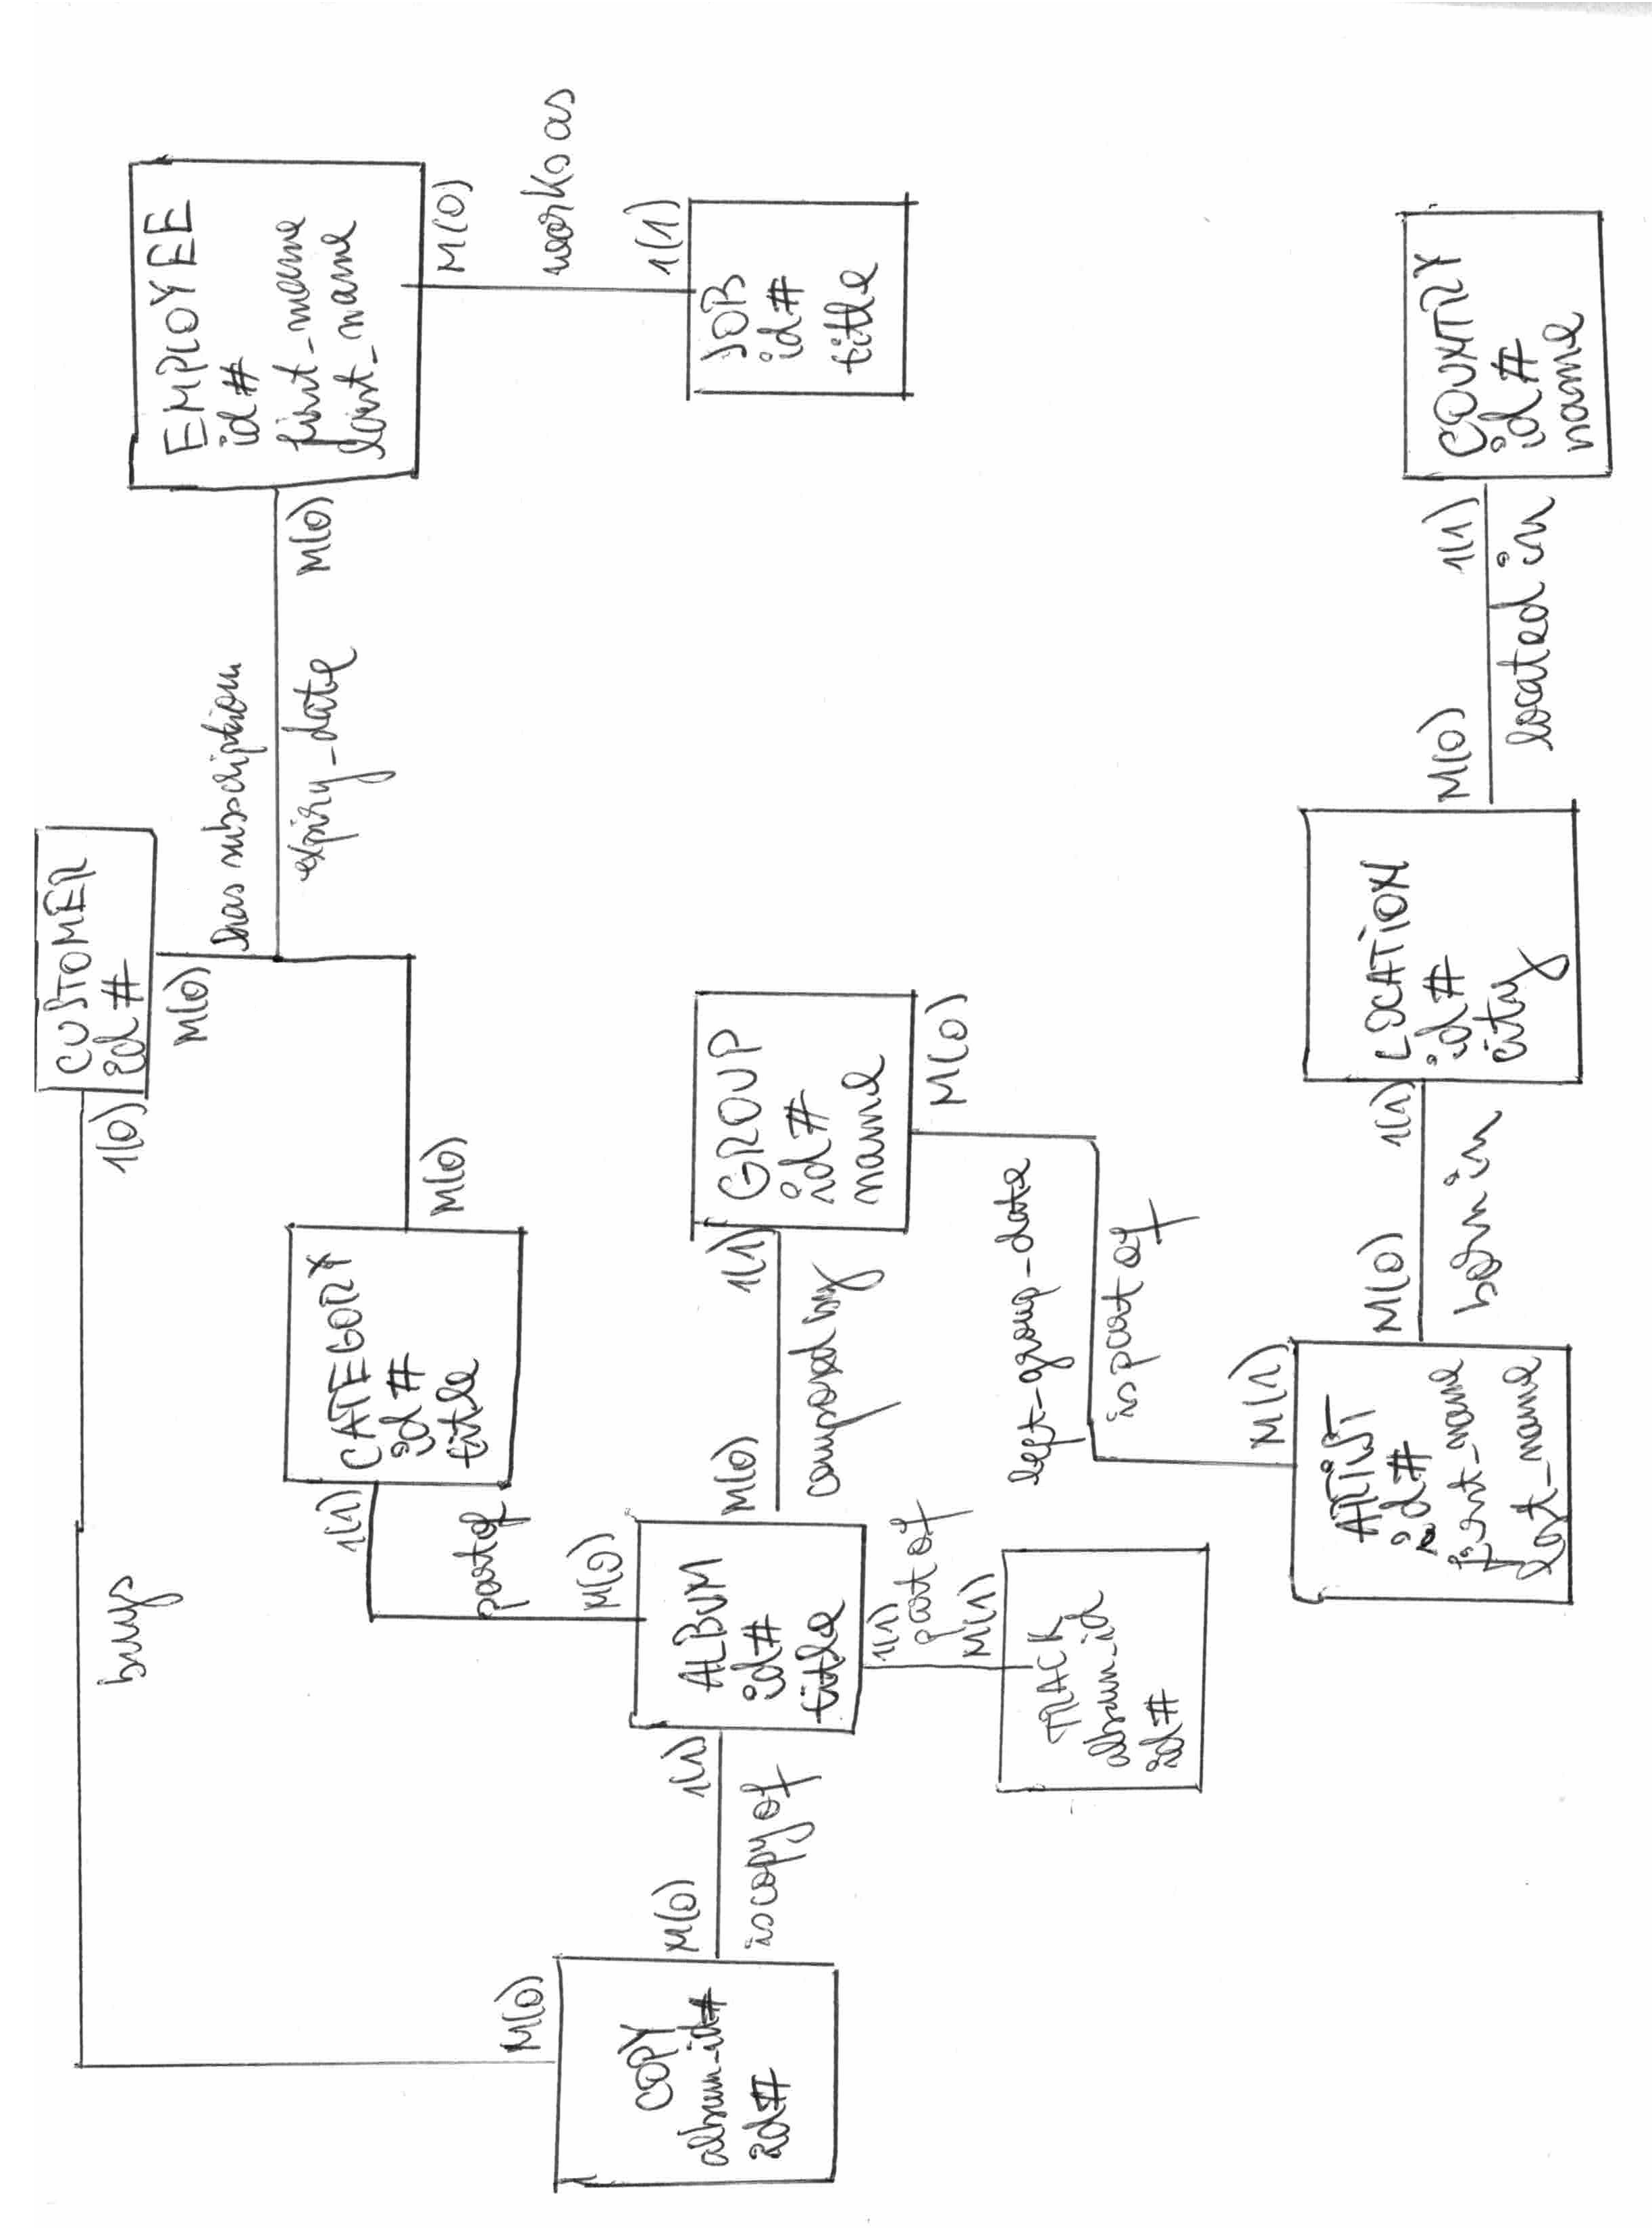
\includepdf[pages=-]{../../img/diagrama_er.png}

\section{Diagrama conceptuală\footnote{pe pagina următoare}}

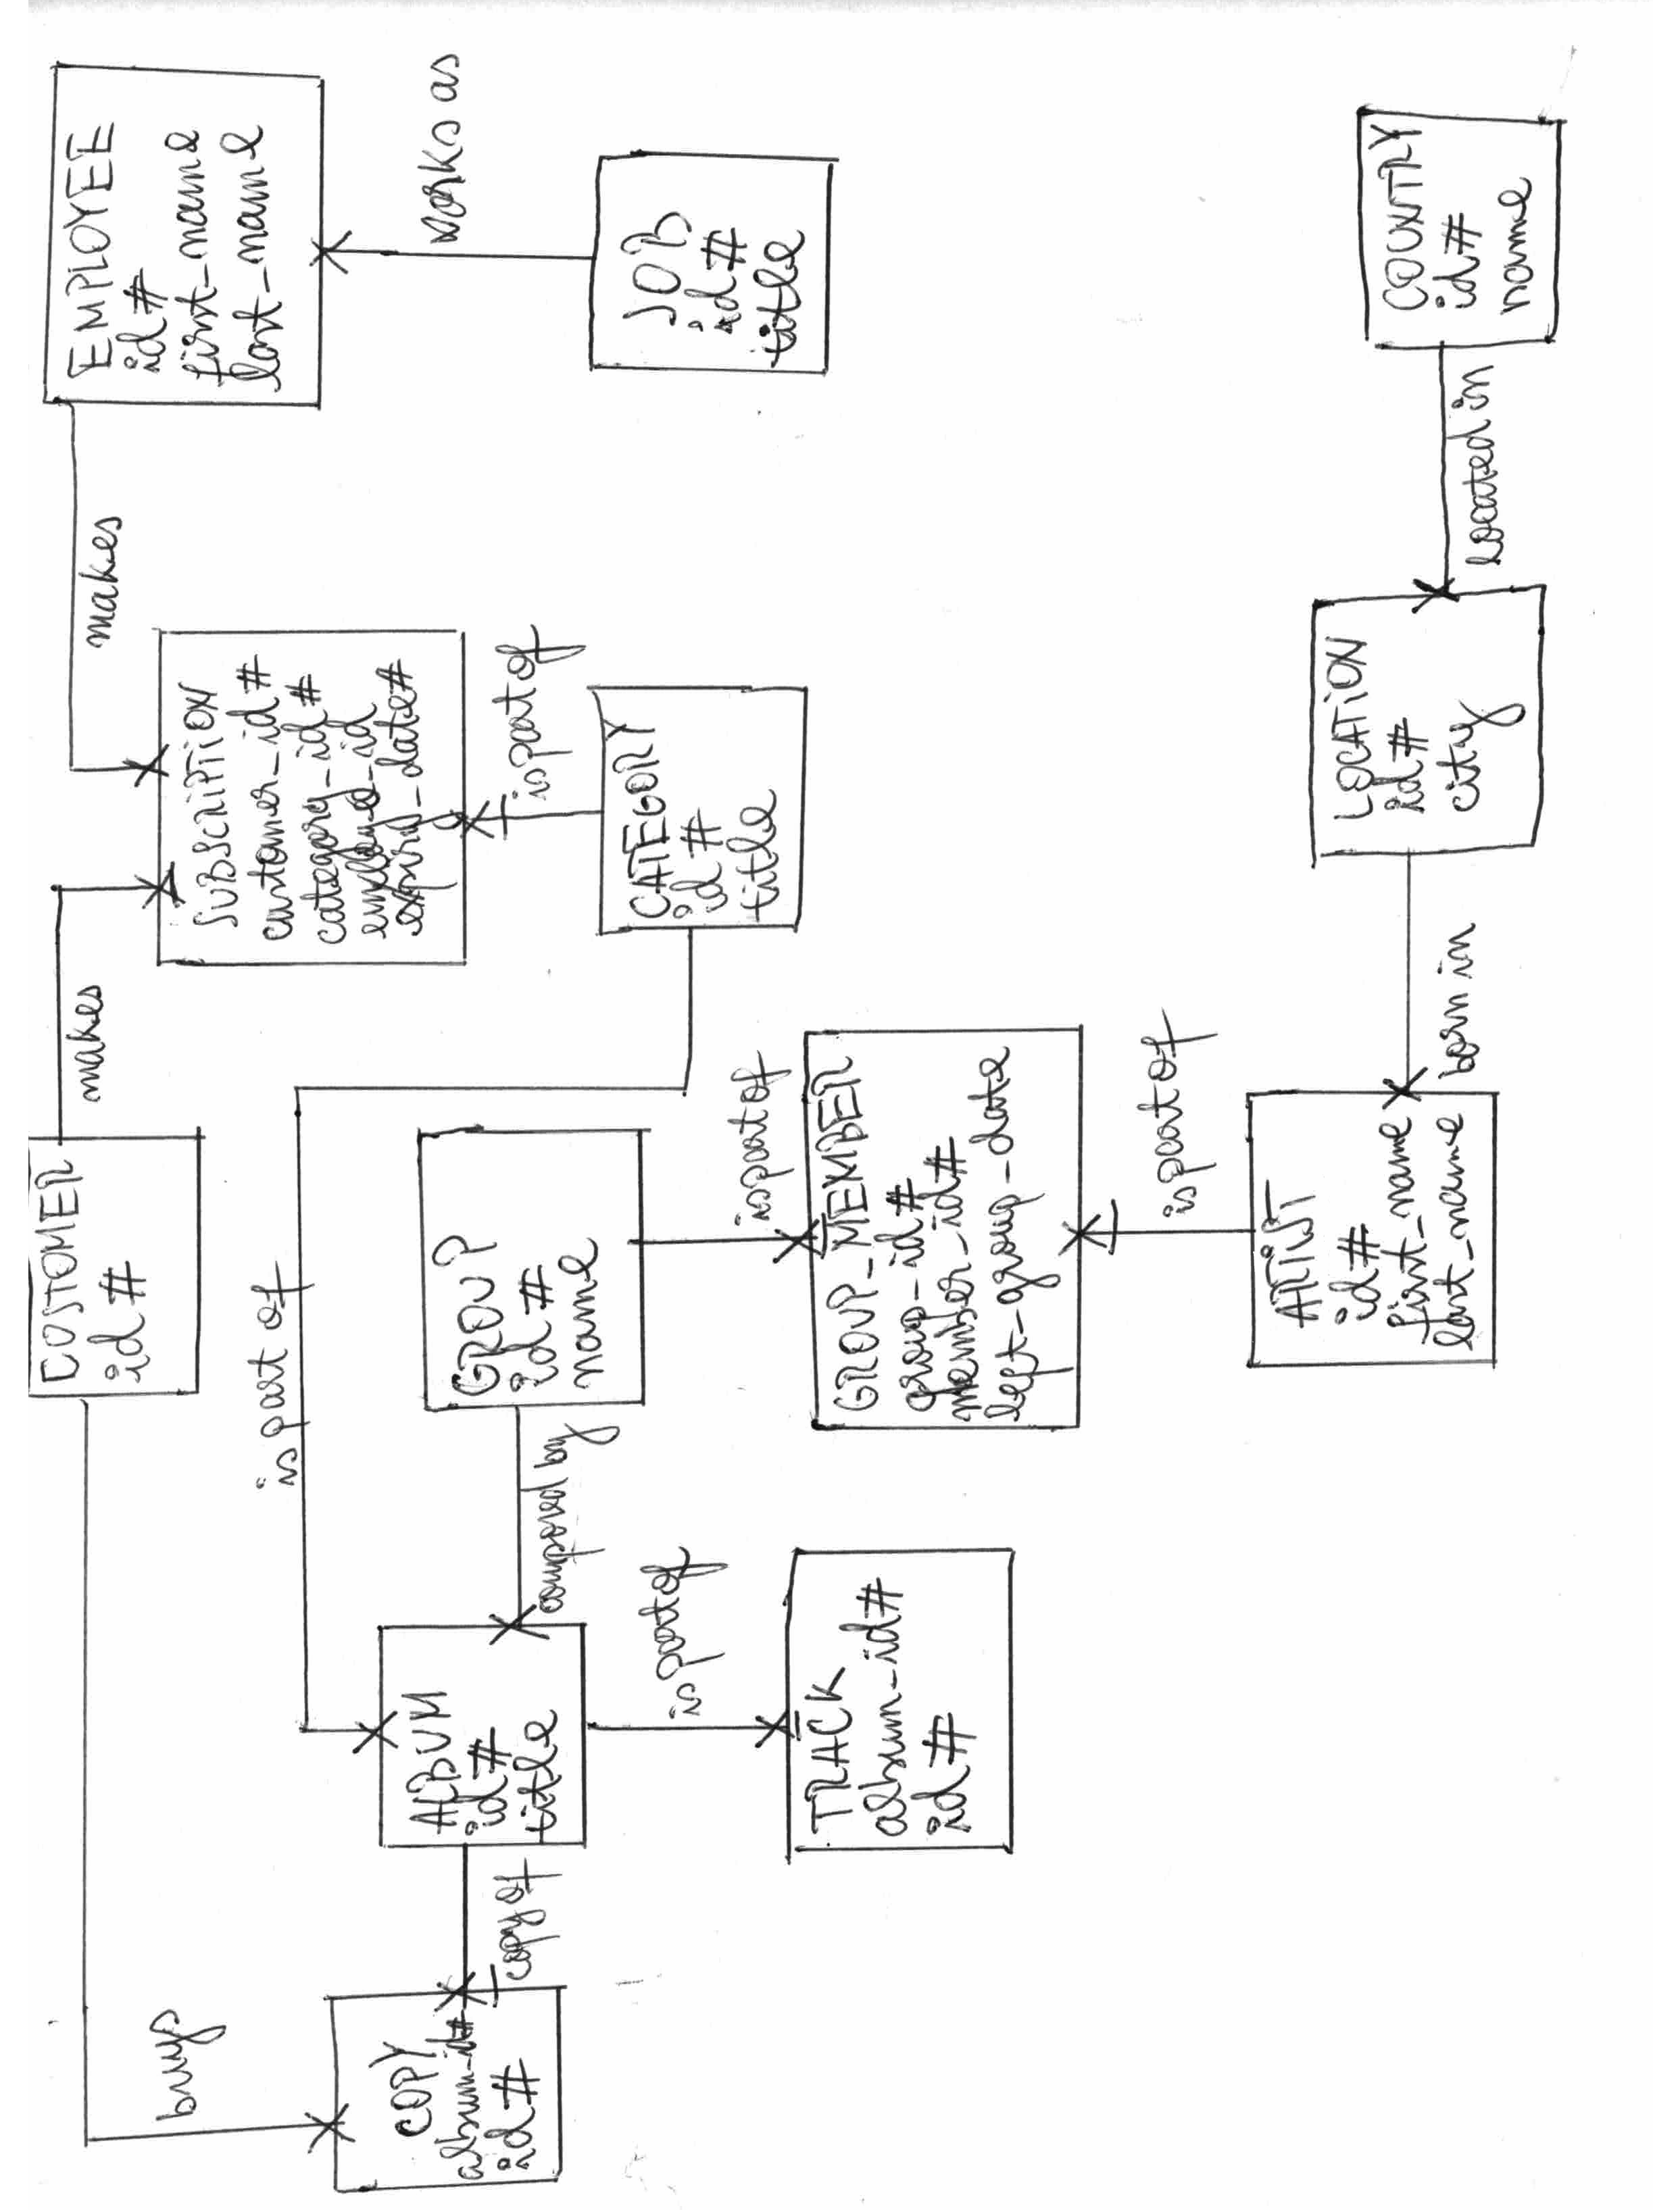
\includepdf[pages=-]{../../img/diagrama_conceptuala.png}

\section{Schemele relaționale}

\begin{center}

\lstinputlisting[language=C]{../../generate/schema_relationala.txt}

\end{center}

\section{Normalizarea până la forma normală 3}

\section{Crearea tabelelor și inserarea de date coerente}

screenshots go here

\section{Cinci cereri SQL complexe}

\begin{center}

\minipage{\linewidth}
\lstinputlisting[caption=\centering{Operație \emph{join} pe minimum 4 tabele{,}
filtrare la nivel de linii{,} subcerere nesincronizată{,} ordonare{,} funcții
pe șiruri de caractere}]{../../queries/1.sql}
\endminipage

\minipage{\linewidth}
\lstinputlisting[caption=\centering{Subcerere sincronizată{,} grupări{,}
funcții grup{,} filtrare la nivel de grupuri{,} operații pe șiruri de
caractere}]{../../queries/2.sql}
\endminipage

\minipage{\linewidth}
\lstinputlisting[caption=\texttt{NVL}{,} \texttt{DECODE}{,} \texttt{CASE}{,}
funcții pe date calendaristice{,} funcții pe șiruri de
caractere]{../../queries/3.sql}
\endminipage

\minipage{\linewidth}
\lstinputlisting[caption=Clauza \texttt{WITH}]{../../queries/4.sql}
\endminipage

\minipage{\linewidth}
\lstinputlisting[caption=Funcții pe date calendaristice]{../../queries/5.sql}
\endminipage

\end{center}

\section{Operații de actualizare/suprimare utilizând subcereri}

\begin{center}

\minipage{\linewidth}
\lstinputlisting[caption=Suprimare/Actualizare utilizând subcereri]{../../queries/6.sql}
\endminipage

\end{center}

\section{Crearea unei secvențe utilizate în inserarea unor înregistrari în tabele}

Secvența următoare este folosită la introducerea datelor în tabela \texttt{Artists}. Generează un ID unic pentru fiecare înregistrare.

\begin{center}

\minipage{\linewidth}
\lstinputlisting[caption=Crearea secvenței]{../../generate/create-sequence.sql}
\endminipage

\minipage{\linewidth}
\lstinputlisting[caption=Exemplu de inserare folosind secvența]{../../generate/sequence-example.sql}
\endminipage

\end{center}

\section{Cerința}
\section{Cerința}

\end{document}
